\chapter{速度の合成、光円錐、四元ベクトル}

\section{一本の線路上の二つの系}

以前に導出したローレンツ変換は、意図的に制限された幾何学に関するものであった。すなわち、すべての相対運動が一つの軸に沿って生じていた。長い線路を思い浮かべよう。一方の観測者集団は駅に留まり、もう一方の観測者集団は線路に沿って動く列車に乗っている。横方向も存在するが、それらが後に復活されるまでは何の役割も果たさない。

各系は操作的に定義された座標系である。その系で静止しているメートル棒が空間座標を定め、その系で静止している同期した時計が時間を定める。両者の関係を確定する公準は、すべての慣性観測者が同じ光速度を測定するというものである。

ほとんどの計算では\(c=1\)を用いる。時間を秒で、距離を光秒で測ってもよいし、年と光年で測ってもよい。その場合、速度は光速度の無次元の割合となる。通常の単位が必要なときは、\(c\)の因子が次元の整合性によって一意に復元される。たとえば、無次元のローレンツ因子における\(v^2\)は\(v^2/c^2\)となる。

\subsection{直接変換と逆変換}

列車の中かその近くのどこかで閃光が起こるとしよう。それは一つの事象であり、誰が記述するかにはよらない。駅の観測者は\((x,t)\)を割り当て、列車の観測者は\((x',t')\)を割り当てる。単位\(c=1\)では、
\begin{align}
x'&=\gamma_v(x-vt),&
t'&=\gamma_v(t-vx),
\label{eq:sr2-direct}\\
\gamma_v&=\frac{1}{\sqrt{1-v^2}}.
\end{align}
ニュートンなら変位\(x-vt\)を認めるであろう。因子\(\gamma_v\)と、\(x\)が\(t'\)に混ざり込むことが相対論的な変更である。

\begin{figure}[htbp]
\centering
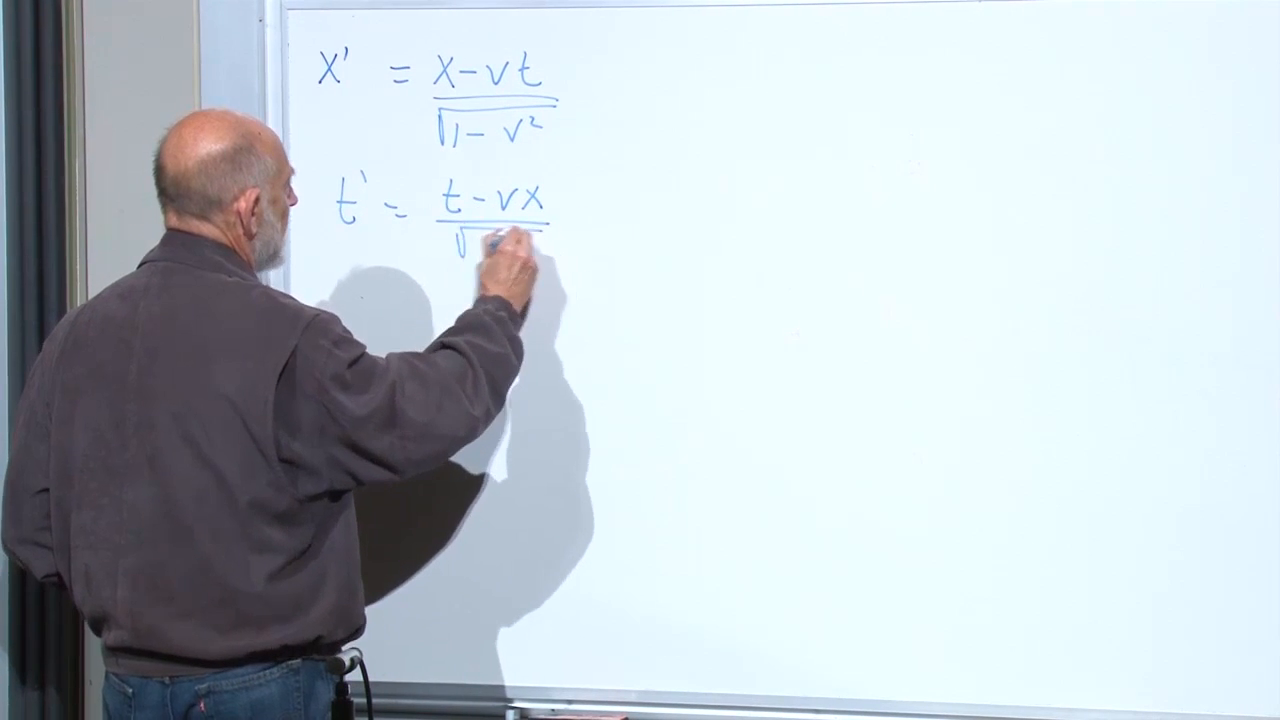
\includegraphics[width=0.90\textwidth]{lecture_02_figure_01.png}
\caption{駅の座標\((x,t)\)と列車の座標\((x',t')\)を関係づける直接ローレンツ変換。}
\lectureframe{00:07:52}
\end{figure}

相反性により、相対速度の符号を反転させれば逆変換が得られる。
\begin{align}
x&=\gamma_v(x'+vt'),&
t&=\gamma_v(t'+vx').
\label{eq:sr2-inverse}
\end{align}
駅は絶対的に静止しているのではない。単にダッシュなしと呼ばれる系であるにすぎず、列車から見れば駅は\(-v\)で動いている。

\begin{figure}[htbp]
\centering
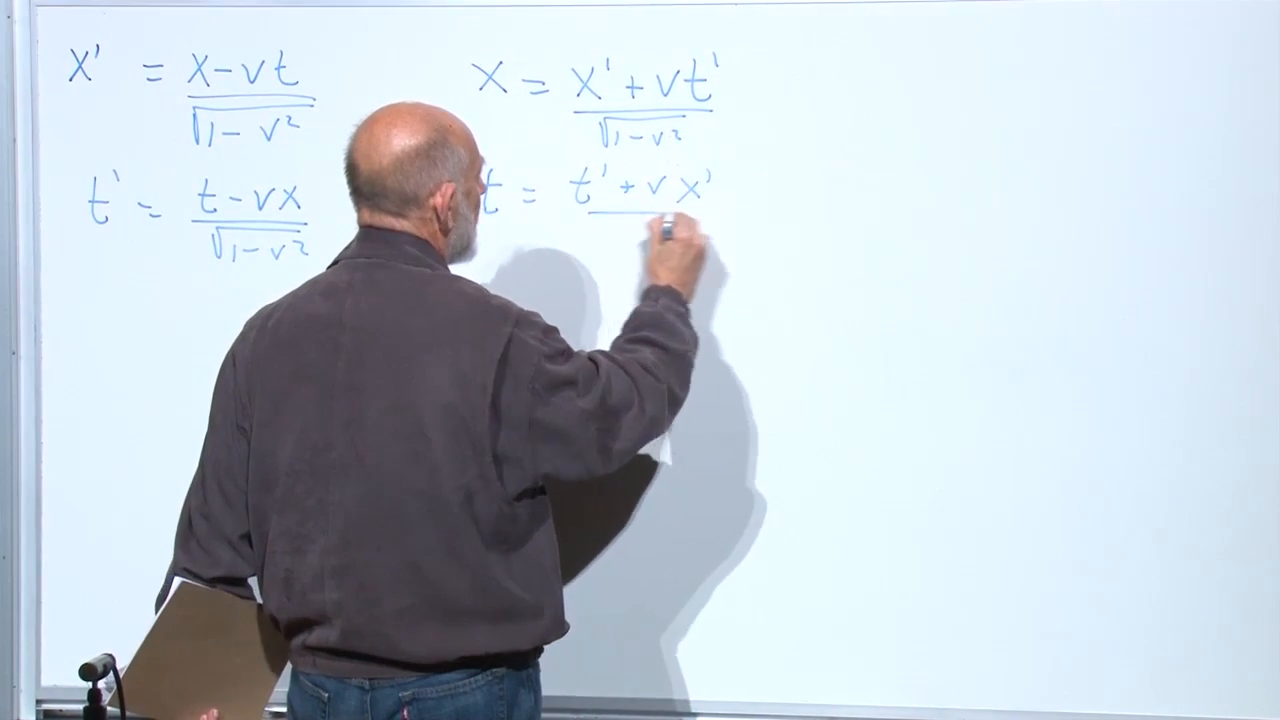
\includegraphics[width=0.90\textwidth]{lecture_02_figure_02.png}
\caption{逆写像は同じローレンツ因子をもち、相対速度の符号は反対である。}
\lectureframe{00:09:15}
\end{figure}

\(x\)に沿ったブーストでは、横方向の座標は変化しない。
\begin{equation}
y'=y,
\qquad
z'=z.
\end{equation}

相対速度は、分母を調べることなく空間の式から読み取ることができる。列車の原点は\(x'=0\)で定義される。したがって
\begin{equation}
x'=0
\quad\Longleftrightarrow\quad
x-vt=0
\quad\Longleftrightarrow\quad
x=vt.
\label{eq:sr2-origin-worldline}
\end{equation}
この世界線における\(t\)の係数が、駅の座標における列車の速さである。

\section{三つの系とブーストの合成}

列車の中に小さなおもちゃの車を置こう。列車は駅に対して速さ\(v\)で動き、車は列車の乗客に対して速さ\(u\)で通路を進む。駅に対する車の速さを\(w\)と呼ぶ。ニュートンの直観は\(w=u+v\)を示唆するが、決めるのはローレンツ変換でなければならない。

ここで三つの座標系が存在する。
\begin{equation}
(x,t),\qquad (x',t'),\qquad (x'',t'').
\end{equation}
第一は駅に、第二は列車に、第三は車に属する。列車と車の間では、
\begin{align}
x''&=\gamma_u(x'-ut'),&
t''&=\gamma_u(t'-ux'),
\label{eq:sr2-second-boost}\\
\gamma_u&=\frac{1}{\sqrt{1-u^2}}.
\end{align}

\begin{figure}[htbp]
\centering
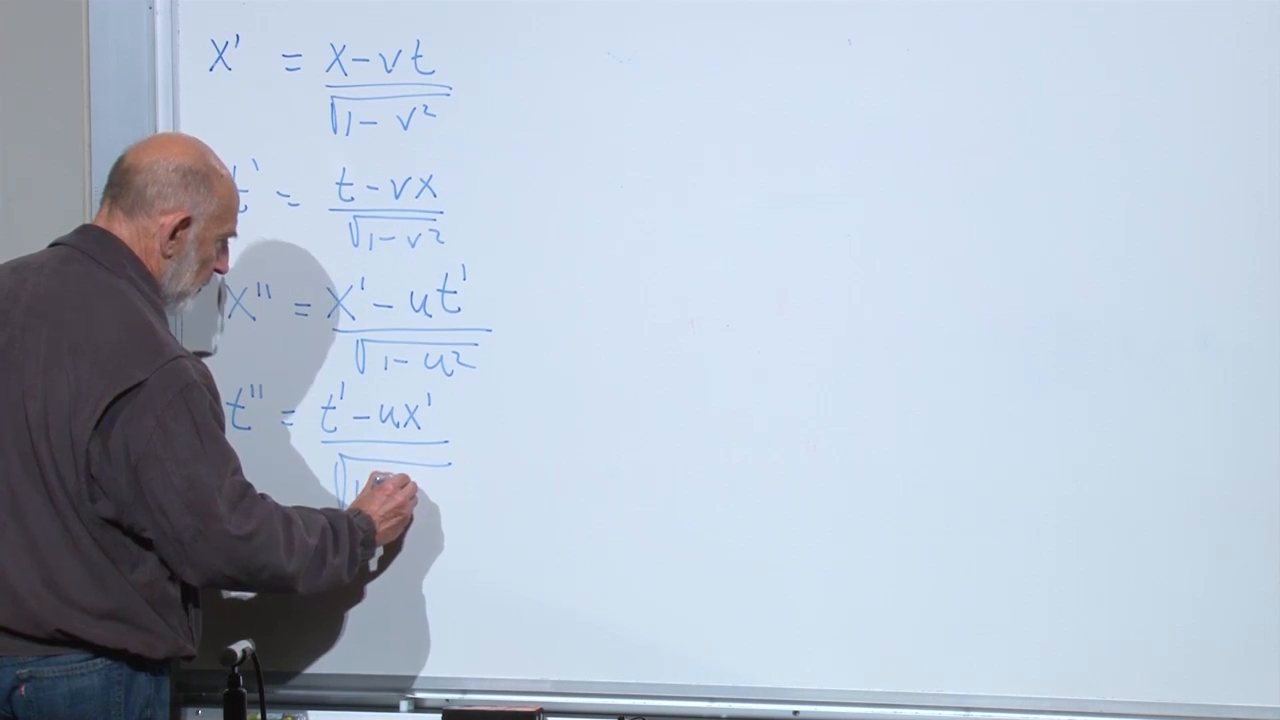
\includegraphics[width=0.90\textwidth]{lecture_02_figure_03.png}
\caption{駅から列車への直接の式に続いて、ダッシュ付きからダッシュ二つの座標への第二のローレンツ変換が行われる。}
\lectureframe{00:14:55}
\end{figure}

\subsection{一方のブーストをもう一方に代入する}

\(w\)を求めるには空間の式で十分である。\eqref{eq:sr2-direct}を\eqref{eq:sr2-second-boost}の第一式に代入すると、
\begin{align}
x''
&=\gamma_u(x'-ut')\\
&=\gamma_u\gamma_v\left[(x-vt)-u(t-vx)\right]\\
&=\gamma_u\gamma_v\left[(1+uv)x-(u+v)t\right].
\label{eq:sr2-composed-space}
\end{align}
\(uvx\)の項にある二つの負号はそれを正にする。二つの時間の項は\(-(u+v)t\)としてまとまる。

\begin{figure}[htbp]
\centering
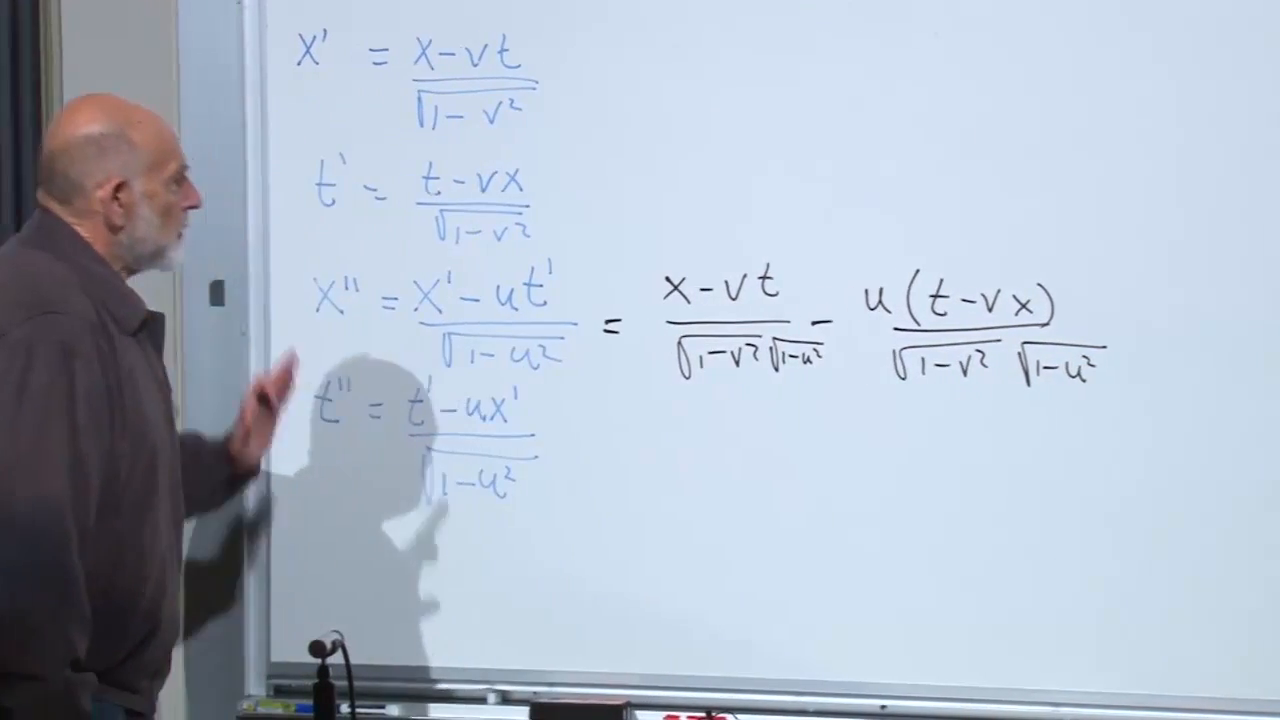
\includegraphics[width=0.91\textwidth]{lecture_02_figure_04.png}
\caption{合成されたブーストにおいて\(x\)項と\(t\)項をまとめる前の、入れ子になった代入。}
\lectureframe{00:16:30}
\end{figure}

以前と同様、動く原点を突き止める際に分母は無関係である。おもちゃの車は\(x''=0\)で静止しているので、\eqref{eq:sr2-composed-space}の括弧はゼロにならなければならない。
\begin{equation}
(1+uv)x-(u+v)t=0.
\end{equation}
したがってその駅系における世界線は
\begin{equation}
x=\frac{u+v}{1+uv}\,t,
\end{equation}
であり、その速度は
\begin{equation}
\boxed{w=\frac{u+v}{1+uv}}.
\label{eq:sr2-velocity-add-c1}
\end{equation}

\begin{figure}[htbp]
\centering
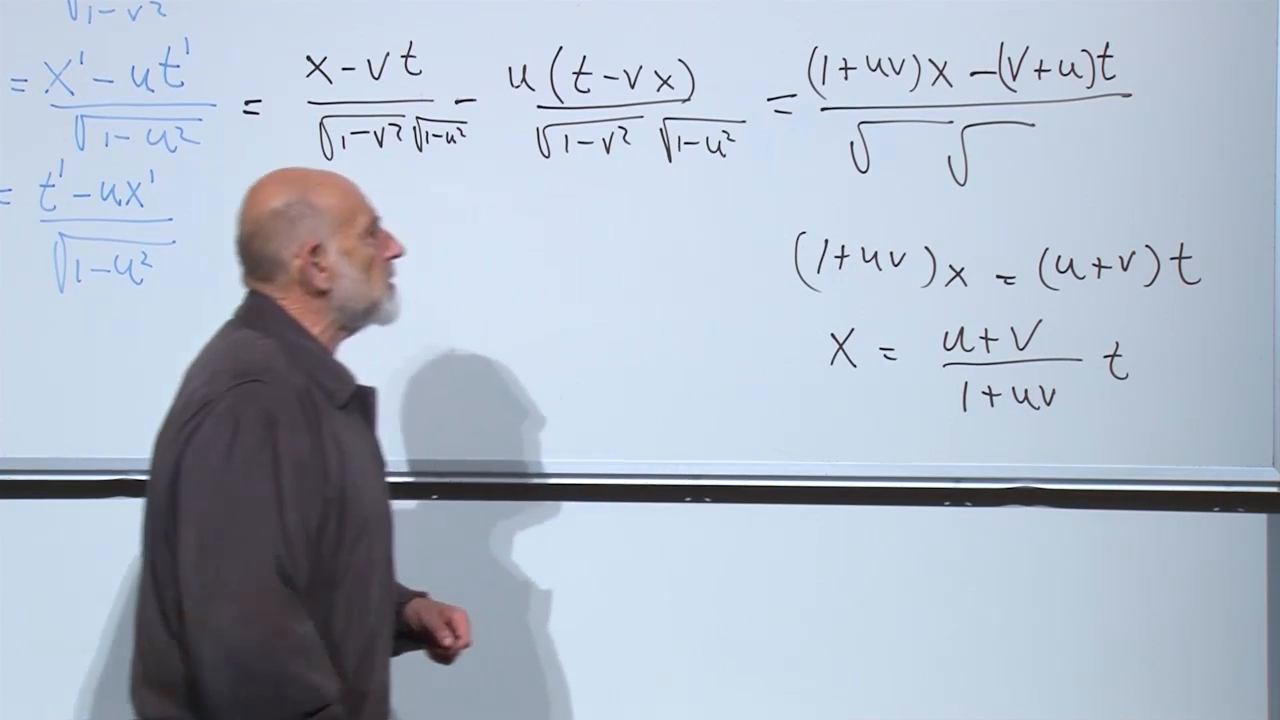
\includegraphics[width=0.91\textwidth]{lecture_02_figure_05.png}
\caption{まとめられた分子と世界線\(x=[(u+v)/(1+uv)]t\)が合成された速度を明らかにする。}
\lectureframe{00:19:30}
\end{figure}

時間の式も整合的に合成される。駅から車への完全な変換はローレンツの形
\begin{align}
x''&=\gamma_w(x-wt),&
t''&=\gamma_w(t-wx),
\end{align}
をもち、ここで
\begin{equation}
\gamma_w=\frac{1}{\sqrt{1-w^2}}.
\end{equation}
である。実際、
\begin{equation}
\gamma_w=\gamma_u\gamma_v(1+uv),
\end{equation}
であり、これは\eqref{eq:sr2-velocity-add-c1}を代入して簡約することにより従う。したがって、二つの共線的なブーストは別の共線的なブーストに合成される。

\subsection{次元の復元}

\begin{classroomqa}
\audiencequestion{通常の単位において、分母\(1+uv\)はなぜ次元的に正しくないのか。}
\lecturerresponse{それが正しいのは、\(c=1\)によってすべての速度が光速度の無次元の割合となるからにすぎない。従来の単位では、この積は\(uv/c^2\)として現れなければならず、これは無次元である。\lecturetimestamp{00:21:11}}
\end{classroomqa}

次元をもつ速度合成則は
\begin{equation}
\boxed{
w=\frac{u+v}{1+\dfrac{uv}{c^2}}
}.
\label{eq:sr2-velocity-add}
\end{equation}

\begin{figure}[htbp]
\centering
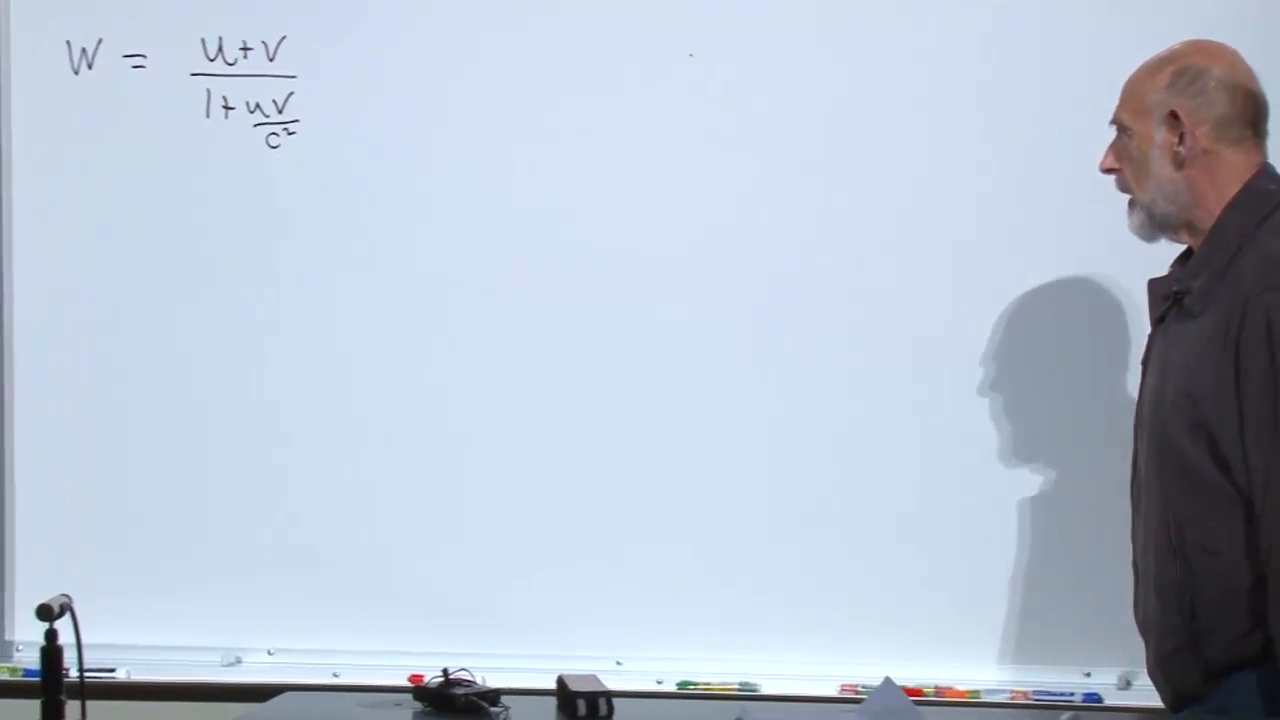
\includegraphics[width=0.90\textwidth]{lecture_02_figure_06.png}
\caption{次元の整合性により、積\(uv\)の下に\(c^2\)が復元される。}
\lectureframe{00:22:06}
\end{figure}

\(\lvert u\rvert,\lvert v\rvert\ll c\)のとき、
\begin{equation}
\frac{uv}{c^2}\ll 1,
\end{equation}
したがって
\begin{equation}
w\approx u+v.
\end{equation}
ニュートン的な合成は、別個の規則ではなく低速近似である。

\subsection{二つの数値的領域}

まず
\begin{equation}
u=v=0.01c.
\end{equation}
をとる。単位\(c=1\)では、
\begin{equation}
w=\frac{0.02}{1.0001}\approx 0.019998.
\end{equation}
光速の1パーセントはすでに約\(3\times10^6\ {\rm m/s}\)であるが、相対論的補正はわずか1万分の1である。結果はニュートン的な\(0.02c\)よりわずかに小さい。

\begin{figure}[htbp]
\centering
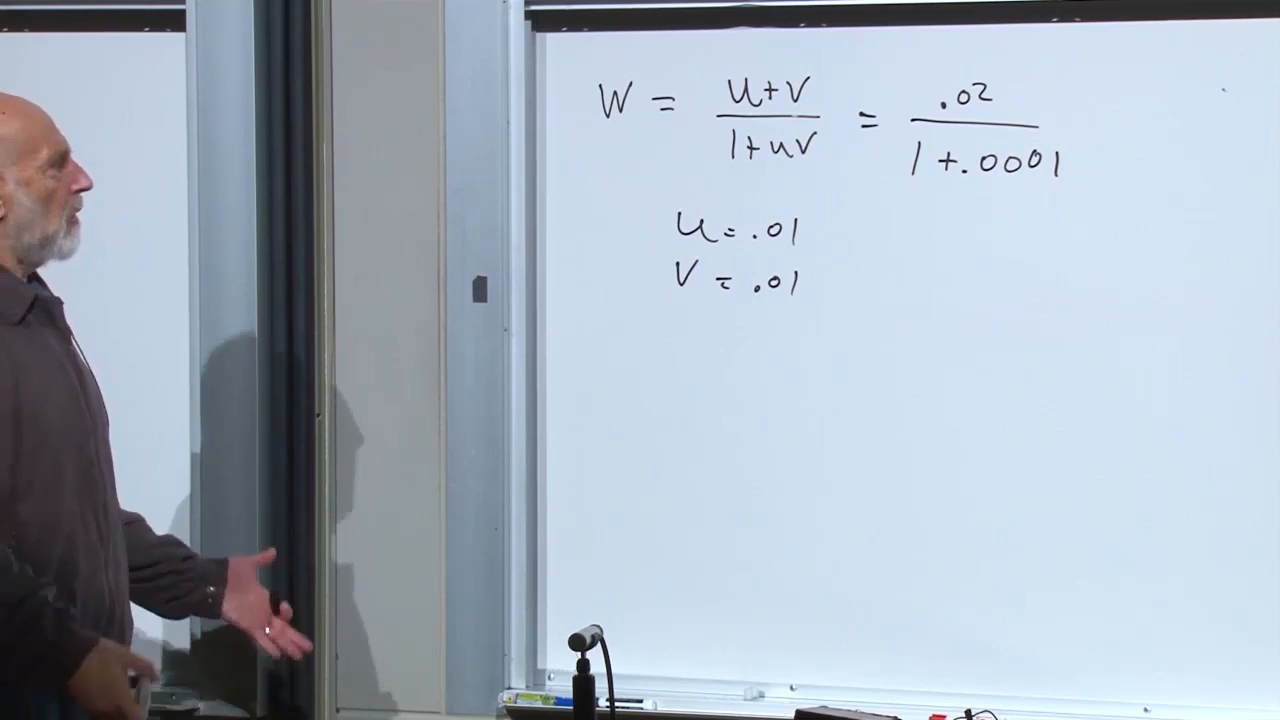
\includegraphics[width=0.90\textwidth]{lecture_02_figure_07.png}
\caption{\(u=v=0.01c\)では、分母は1からわずか\(10^{-4}\)だけ異なる。}
\lectureframe{00:24:23}
\end{figure}

次に
\begin{equation}
u=v=0.9c.
\end{equation}
をとる。ニュートンなら\(1.8c\)と予測するであろう。相対論では
\begin{equation}
\frac{w}{c}
=\frac{0.9+0.9}{1+0.9^2}
=\frac{1.8}{1.81}
\approx 0.9945.
\label{eq:sr2-fast-example}
\end{equation}
を与える。

\begin{figure}[htbp]
\centering
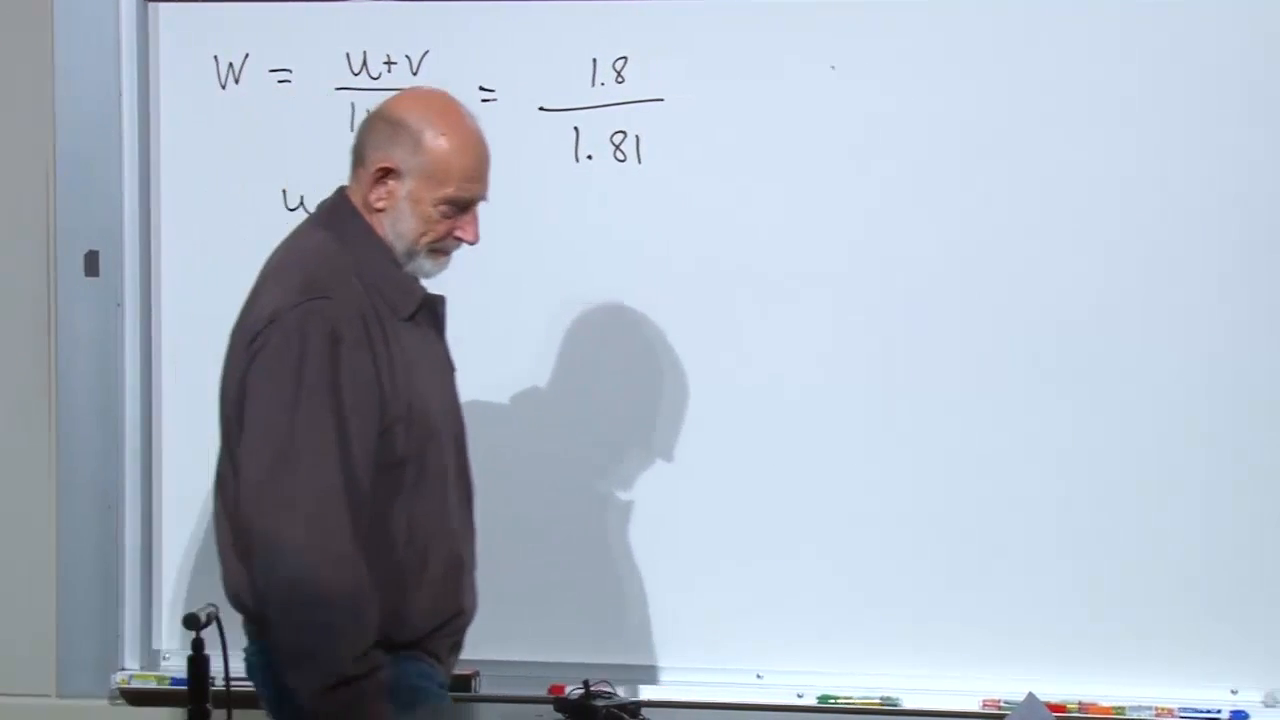
\includegraphics[width=0.90\textwidth]{lecture_02_figure_08.png}
\caption{\(0.9c\)の二つの速度は\(1.8/1.81\)に合成され、依然として光速より小さい。}
\lectureframe{00:25:48}
\end{figure}

光速以下のブーストを繰り返しても\(c\)を越えることはできない。\(u<c\)かつ\(v<c\)ならば、
\begin{equation}
1-\frac{w}{c}
=
\frac{\left(1-\frac{u}{c}\right)
      \left(1-\frac{v}{c}\right)}
     {1+\frac{uv}{c^2}}
>0.
\end{equation}
ブーストを追加するごとに結果を\(c\)に近づけることはできるが、それを越えることは決してない。極限値\(u=c\)では、
\begin{equation}
w=\frac{c+v}{1+v/c}=c.
\end{equation}
光速は合成則の固定点である。

\section{座標測定は視覚的見え方ではない}

\begin{classroomqa}
\audiencequestion{列車にガラス張りの壁があるなら、駅の観測者は単に乗客と子供用車を一緒に見て、それらの運動を直接読み取れるのだろうか。}
\lecturerresponse{ローレンツ変換が扱うのは、配置された棒と同期した時計によって行われる座標測定である。視覚的像には、異なる事象から観測者に至る光の伝播時間が等しくないことも含まれる。ガラスは見え方を変えるが座標関係を変えるものではなく、一つの像を同時的なデータとして扱えば、相対論がまさに修正した同時性の仮定を再導入することになる。\lecturetimestamp{00:27:53}}
\end{classroomqa}

事象は、その瞬間に誰かがそれを見るかどうかに関係なく、各座標系において位置と時刻をもつ。光学的見え方は正当な主題であるが、各事象から目に至る光を追跡する第二の計算を必要とする。変換則それ自体は普遍的であり、列車の壁とは無関係である。

\section{三次元空間における固有間隔}

二つの事象に戻る。最初は一方が原点にあり、他方が\((x,t)\)にあるとする。一次元空間では、
\begin{equation}
\tau^2=t^2-x^2
\label{eq:sr2-interval-1d}
\end{equation}
単位\(c=1\)で表される。すべての慣性系が一致する：
\begin{equation}
\tau^2
=t^2-x^2
=t'^2-x'^2
=t''^2-x''^2.
\end{equation}
座標は変化するが、固有間隔は変化しない。

時間的隔たりの場合、時計は事象間を移動できる。最初の事象で正午を示すなら、二番目の事象におけるその経過表示は固有時\(\tau\)である。この記述は、間隔を計算するためにどの座標系を用いるかとは独立である。

\begin{figure}[htbp]
\centering
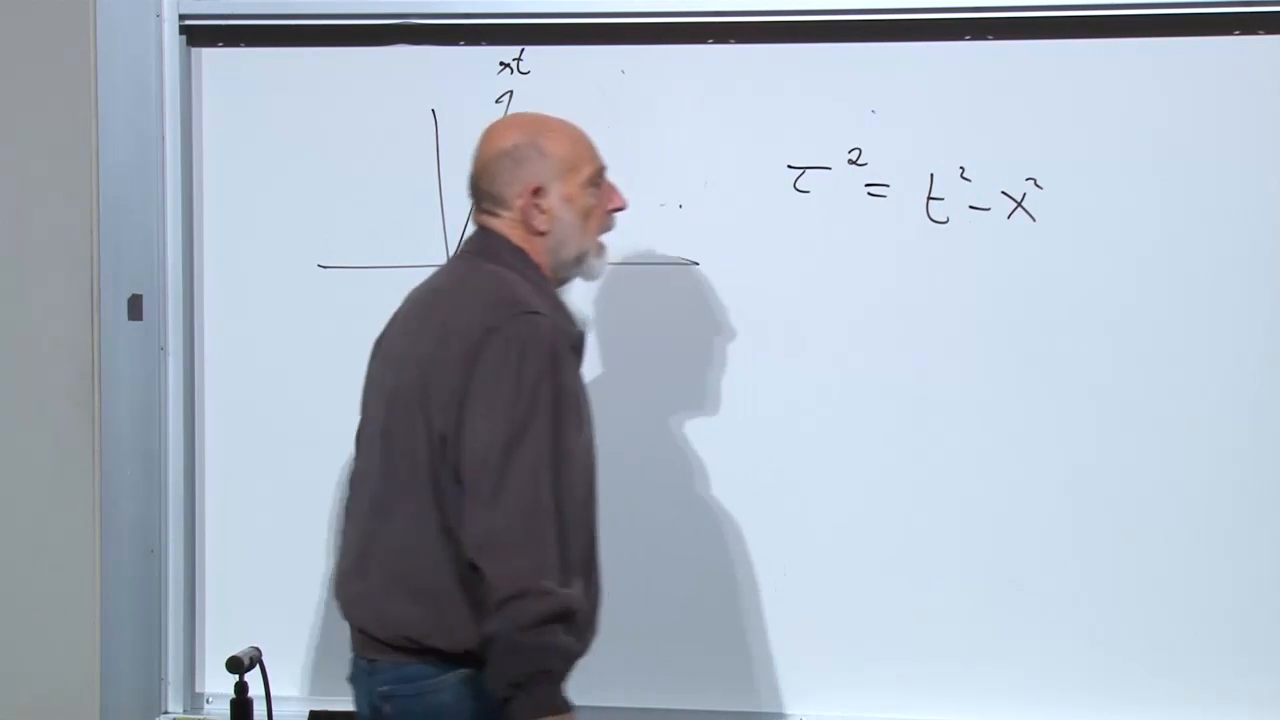
\includegraphics[width=0.90\textwidth]{lecture_02_figure_09.png}
\caption{不変な固有時関係\(\tau^2=t^2-x^2\)は、横方向を復元する前に思い出される。}
\lectureframe{00:30:18}
\end{figure}

\subsection{空間的回転が横方向を復元する}

ブーストに戻る前に、空間軸の通常の回転を考える。\(x\)軸上にない点は、空間的距離の二乗
\begin{equation}
r^2=x^2+y^2+z^2,
\end{equation}
をもち、これは通常のピタゴラスの定理により回転の下で不変である。したがって\(3+1\)次元時空間間隔は
\begin{equation}
\boxed{
\tau^2=t^2-x^2-y^2-z^2
}.
\label{eq:sr2-interval-3d}
\end{equation}
となる。\(c\)を復元すると、
\begin{equation}
c^2\tau^2
=c^2t^2-x^2-y^2-z^2.
\end{equation}

\begin{figure}[htbp]
\centering
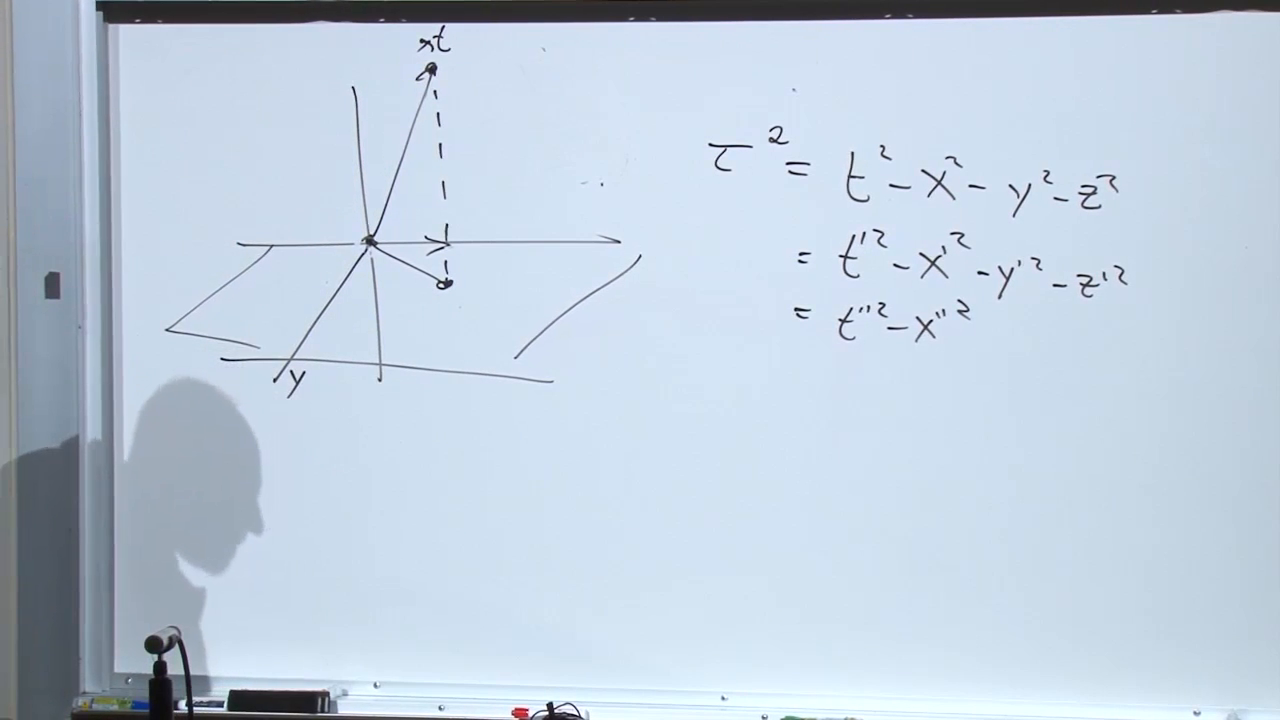
\includegraphics[width=0.90\textwidth]{lecture_02_figure_10.png}
\caption{ピタゴラス的空間距離が不変量を\(t^2-x^2\)から\(t^2-x^2-y^2-z^2\)へ拡張する。}
\lectureframe{00:34:23}
\end{figure}

空間的回転とローレンツブーストの任意の組み合わせが\eqref{eq:sr2-interval-3d}を保存する。通常の座標軸は成分について一致しないがユークリッド距離について一致する。慣性時空間系は空間成分と時間成分について一致しないが、この二乗の差について一致する。その不変量が特殊相対性理論の中心的な幾何学的事実である。

\begin{classroomqa}
\audiencequestion{乗客が子供用車を前方への懐中電灯の光線に置き換えたなら、列車の観測者と駅の観測者は同じ光速を得るだろうか。}
\lecturerresponse{\eqref{eq:sr2-velocity-add}において\(u=c\)と置く。すると\(w=(c+v)/(1+v/c)=c\)となる。\(c=1\)単位では比は単に\((1+v)/(1+v)=1\)である。両方の系が同じ速さを測定し、まさに要求どおりである。\lecturetimestamp{00:35:53}}
\end{classroomqa}

したがって、先のガラス壁の懸念は不変な光速の失敗ではない。それは座標測定と遅延した視覚的像との混同であり、究極的には同時性についての混同である。

\section{ヌル光線と光円錐}

一次元空間では、右向きおよび左向きに進む光線は
\begin{equation}
x=\pm t.
\end{equation}
を満たす。それらの間隔は消える：
\begin{equation}
t^2-x^2=0.
\end{equation}
ユークリッド距離とは異なり、時空間間隔がゼロであることは事象が一致することを要求しない。それは光信号がそれらを結びうることを意味する。

すべての空間方向が復元されると、光線は
\begin{equation}
t^2-x^2-y^2-z^2=0,
\label{eq:sr2-null}
\end{equation}
または
\begin{equation}
r=t
\end{equation}
を満たす。ここで \(c=1\) 単位における未来向きの光を考えている。

\begin{figure}[htbp]
\centering
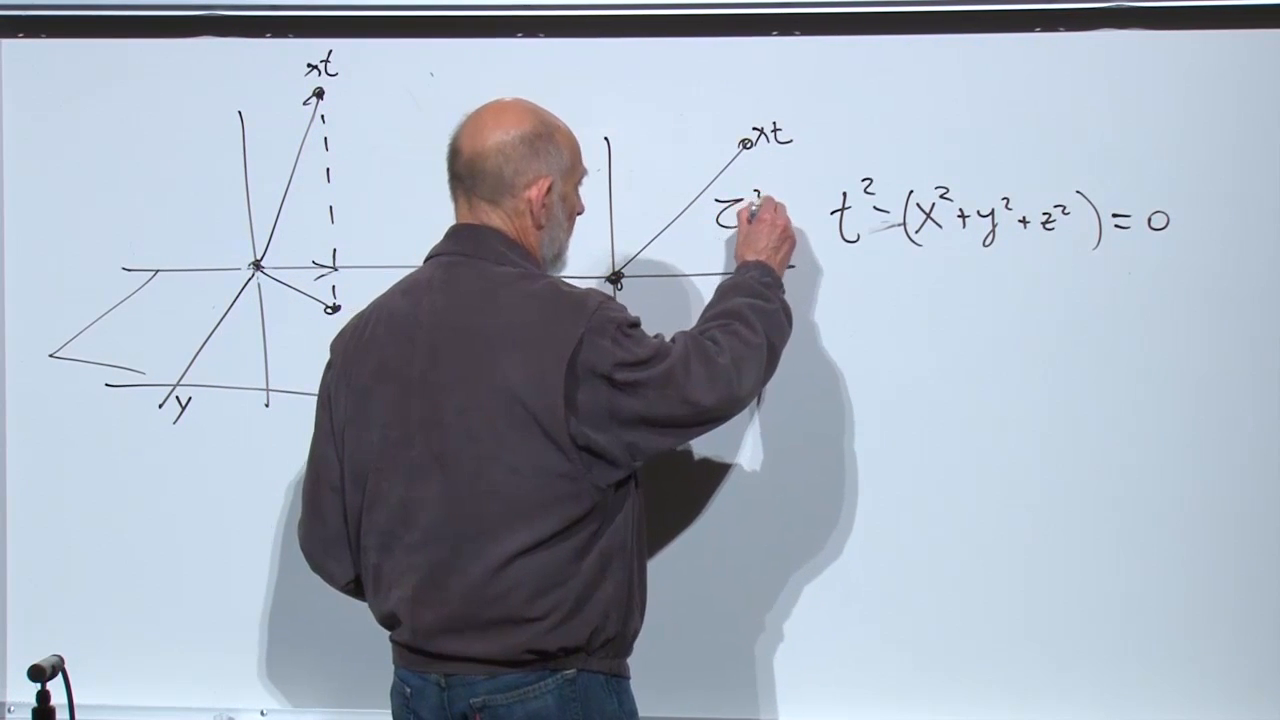
\includegraphics[width=0.90\textwidth]{lecture_02_figure_11.png}
\caption{任意の空間方向の光は \(t^2-(x^2+y^2+z^2)=0\) を満たすヌル軌道に従う。}
\lectureframe{00:39:28}
\end{figure}

\(1+1\) 次元では、ヌル集合は一対の \(45^\circ\) 直線である。空間2次元に時間を加えると円錐になり、空間3次元は黒板に完全には描けないが、定義方程式は変わらない。

未来光円錐は、原点で放出された光が到達しうる事象からなる。過去光円錐は、そこから光が原点に到達しうる事象からなる。一方は他方を時間的にひっくり返したものである。

\begin{figure}[htbp]
\centering
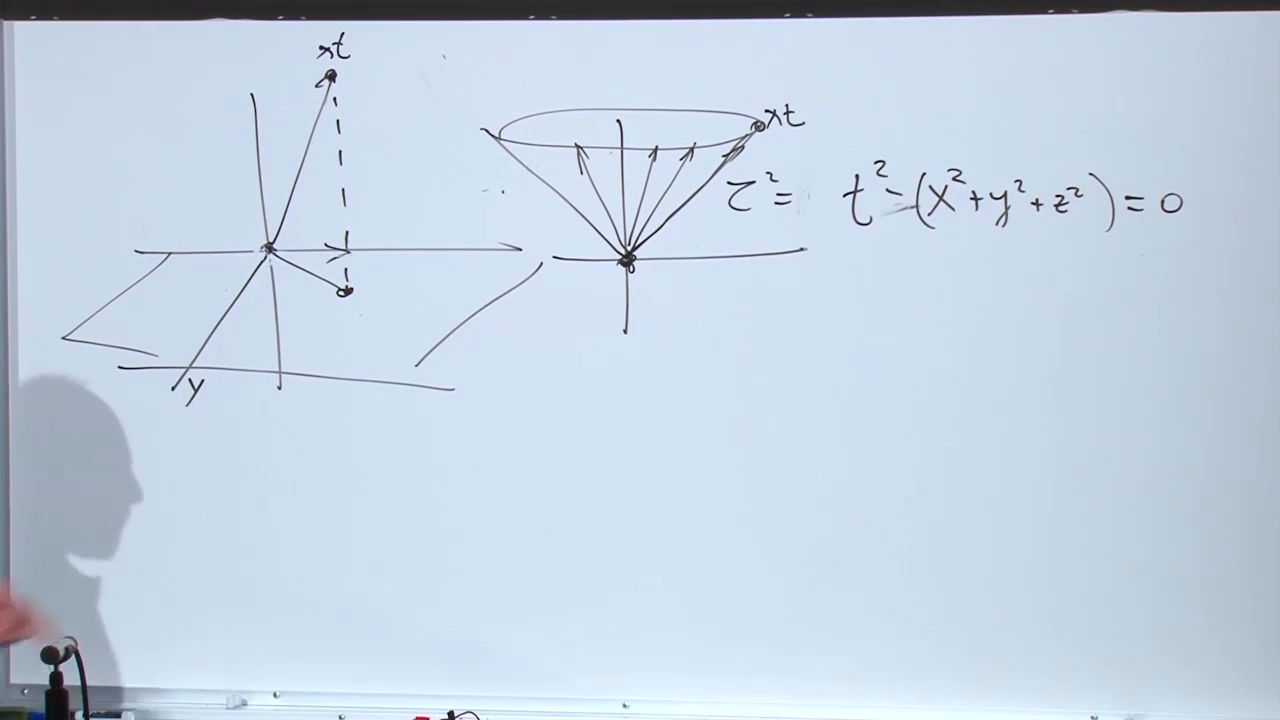
\includegraphics[width=0.90\textwidth]{lecture_02_figure_12.png}
\caption{\(45^\circ\) のヌル光線は、より高次元の時空図において未来光円錐と過去光円錐を掃き出す。}
\lectureframe{00:40:47}
\end{figure}

\begin{classroomqa}
\audiencequestion{ニュートン力学においてガリレイ変換の下で対応する不変量は何か。}
\lecturerresponse{時間間隔そのものである。ニュートン的な観測者は、空間的変位については一致しないが、\(\Delta t\) については皆一致する。相対性理論は普遍時間を放棄し、それを不変な時空間隔で置き換える。\lecturetimestamp{00:41:53}}
\end{classroomqa}

\section{空間ベクトルから四元ベクトルへ}

ここでのベクトルは幾何学的ベクトルであり、量子状態ベクトルではない。通常空間における2点間の変位は大きさと向きをもつ。その始点はベクトルを変えずに原点へ平行移動でき、その3成分は
\begin{equation}
x^i=(x^1,x^2,x^3)=(x,y,z),
\qquad i=1,2,3.
\end{equation}
と表せる。ラテン添字 \(i\) は空間方向のみを走る。

事象には、その時刻という成分がもう一つ必要である。したがって時空の位置は
\begin{equation}
x^\mu=(x^0,x^1,x^2,x^3)=(t,x,y,z),
\qquad \mu=0,1,2,3.
\label{eq:sr2-four-position}
\end{equation}
と書かれる。歴史的な慣習により、時間は四番目ではなく零番目の成分である：
\begin{equation}
x^0=t,\qquad x^1=x,\qquad x^2=y,\qquad x^3=z.
\end{equation}
\(\mu\) のようなギリシア文字の添字は時空全体にわたり、\(i\) のようなラテン文字の添字は空間にわたる。

\begin{figure}[htbp]
\centering
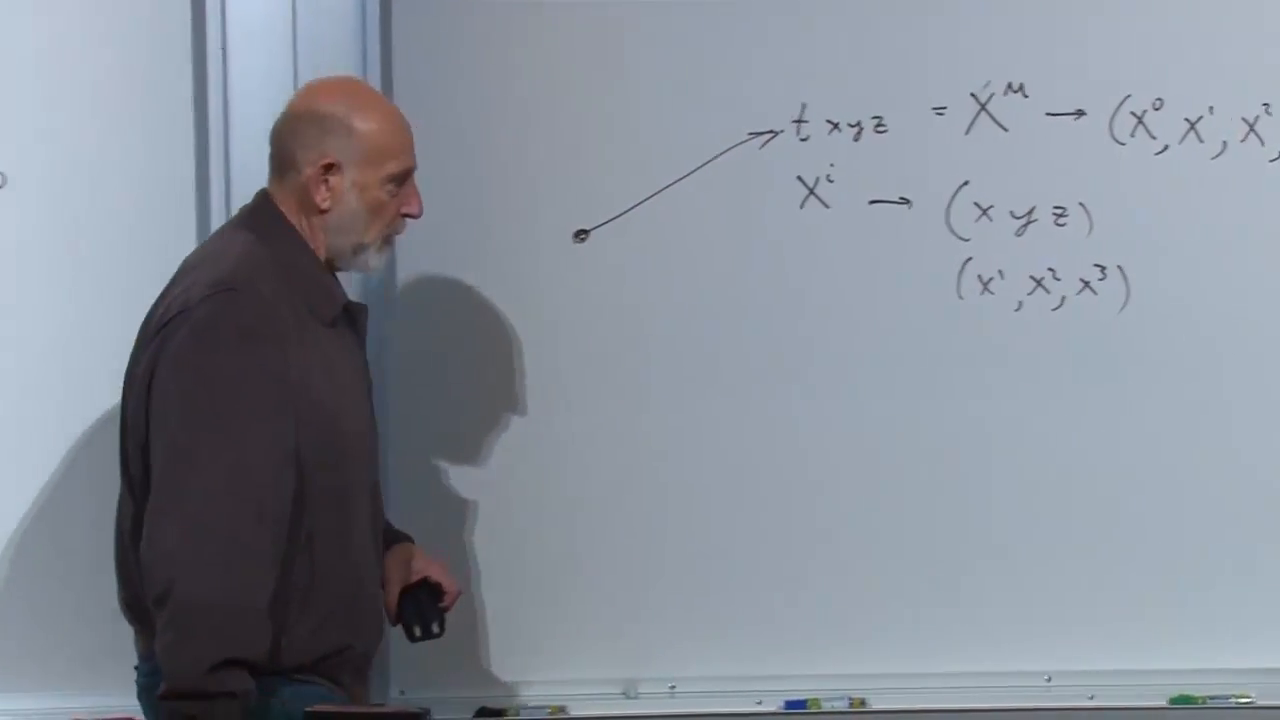
\includegraphics[width=0.90\textwidth]{lecture_02_figure_13.png}
\caption{空間成分 \(x^i\) は4成分の時空位置 \(x^\mu=(x^0,x^1,x^2,x^3)\) に拡張される。}
\lectureframe{00:46:05}
\end{figure}

不変量は
\begin{equation}
\tau^2
=(x^0)^2-(x^1)^2-(x^2)^2-(x^3)^2.
\end{equation}
となる。記法だけでは新しい物理は何も加わらない。その価値は、ローレンツ変換が回転が空間ベクトルに線形に作用するのとちょうど同じように、4つの成分すべてに線形に作用することにある。

\begin{classroomqa}
\audiencequestion{変換が線形であるから、列ベクトルに作用する行列で表せるか。}
\lecturerresponse{はい。\(x\) に沿ったブーストでは、非自明なブロックは \((t,x)^{\mathsf T}\) に作用する \(\gamma_v\begin{pmatrix}1&-v\\-v&1\end{pmatrix}\) であり、\(y\) と \(z\) は変わらない。行列記法はローレンツ変換を合成し整理する自然な方法である。\lecturetimestamp{00:48:14}}
\end{classroomqa}

陽に書けば、
\begin{equation}
\begin{pmatrix}
t'\\x'\\y'\\z'
\end{pmatrix}
=
\begin{pmatrix}
\gamma_v&-\gamma_v v&0&0\\
-\gamma_v v&\gamma_v&0&0\\
0&0&1&0\\
0&0&0&1
\end{pmatrix}
\begin{pmatrix}
t\\x\\y\\z
\end{pmatrix}.
\label{eq:sr2-boost-matrix}
\end{equation}

\section{変位と四元速度}

一つの事象の位置から、粒子の世界線の短い線分へ移ろう。四元変位は
\begin{equation}
\Delta x^\mu
=(\Delta t,\Delta x,\Delta y,\Delta z).
\end{equation}
である。変位が小さいと呼ばれるとき、微積分が近づいている：\(\Delta x^\mu\) は \(dx^\mu\) になるであろう。今のところ、有限の記法が幾何学を透明にする。

時間的 worldline に沿った固有時間の増分は
\begin{equation}
(\Delta\tau)^2
=(\Delta t)^2-(\Delta x)^2-(\Delta y)^2-(\Delta z)^2.
\label{eq:sr2-proper-increment}
\end{equation}
を満たす。通常の速度は空間変位を座標時間で割り、3つの成分をもつ。四元速度は代わりに四元変位を不変な固有時間で割る：
\begin{equation}
u^\mu
=\frac{\Delta x^\mu}{\Delta\tau}
\quad\longrightarrow\quad
\boxed{
u^\mu=\frac{dx^\mu}{d\tau}
}.
\label{eq:sr2-four-velocity}
\end{equation}

\begin{figure}[htbp]
\centering
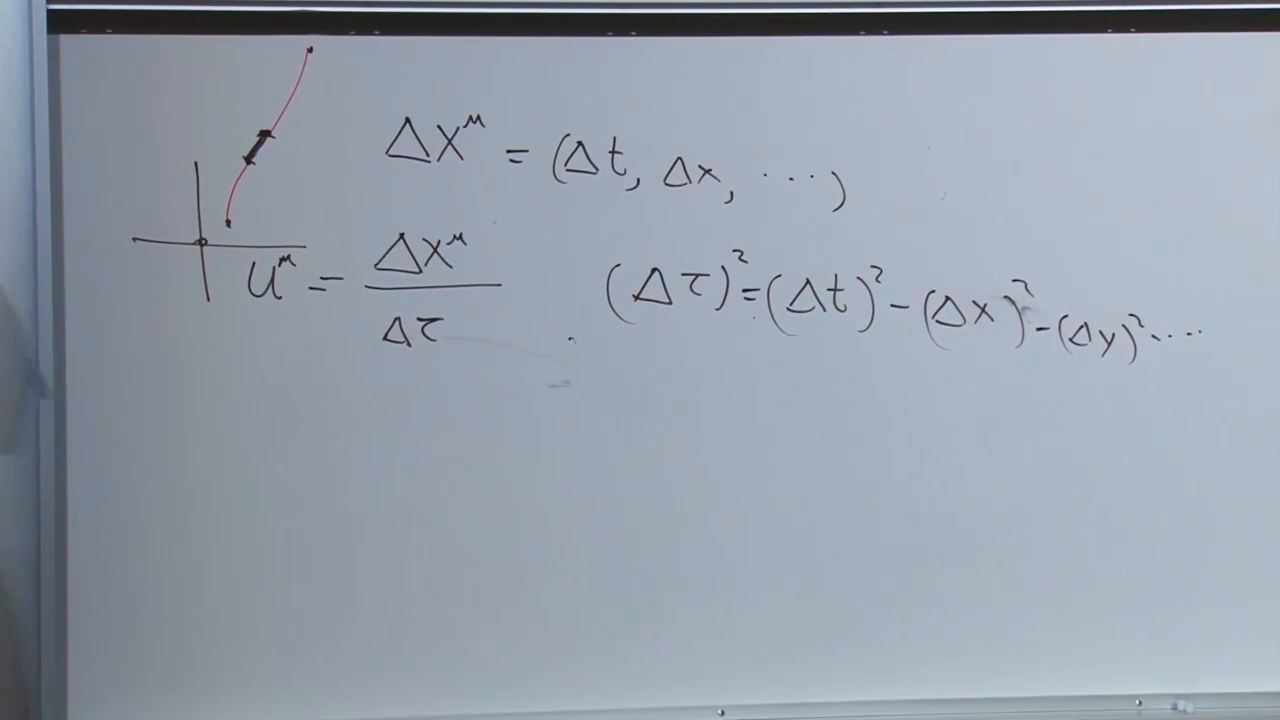
\includegraphics[width=0.90\textwidth]{lecture_02_figure_14.png}
\caption{世界線の線分は \(\Delta x^\mu\)、その不変量 \(\Delta\tau\)、および四元速度 \(u^\mu=\Delta x^\mu/\Delta\tau\) を定義する。}
\lectureframe{00:52:42}
\end{figure}

この対象は4つの成分をもち、四元ベクトルとして変換する。それが通常の3次元速度とどう関係するかが次の問いであり、ここでは意図的に未解決のままにしておく。これを解決することは、相対論的運動量、エネルギー、加速度、そして最終的には \(F=ma\) の相対論的一般化へと導く。